\section{Einleitung}
Dies soll eine \LaTeX{}-Vorlage für den persönlichen Gebrauch werden. Sie hat weder einen Anspruch auf Richtigkeit, noch auf Vollständigkeit. Die Quellen liegen auf Github zur allgemeinen Verwendung. Verbesserungen sind jederzeit willkommen.

\subsection{Zielsetzung}
Kleiner Reminder für mich in Bezug auf die Dinge, die wir bei der Thesis beachten sollten und \LaTeX{}-Vorlage für die Thesis.

\subsection{Aufbau der Arbeit}
Kapitel \ref{infos} enthält die Inhalte des Thesis-Days und alles, was zum inhaltlichen erstellen der Thesis relevant sein könnte. In Kapitel \ref{latexDetails} \nameref{latexDetails} findet ihr wichtige Anmerkungen zu \LaTeX{}, wobei die wirklich wichtigen Dinge im Quelltext dieses Dokumentes stehen (siehe auch die Verzeichnisstruktur in Abbildung \ref{fig:verzeichnisStruktur}).


\begin{figure}[H]
 \centerline{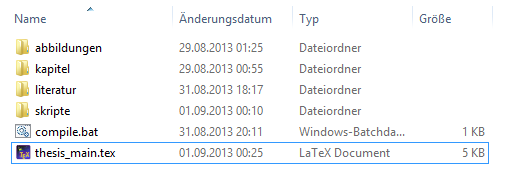
\includegraphics[width=0.9\textwidth]{verzeichnisStruktur}}
 \caption{Verzeichnisstruktur der \LaTeX{}-Datein}\label{fig:verzeichnisStruktur}
 \floatfoot{Quelle: Eigene Darstellung}
\end{figure}
